\documentclass[../main/main.tex]{subfiles}
\begin{document}
%\dominitoc
%\faketableofcontents
\setcounter{chapter}{2}
\chapter{Zwicky Transient Facility}\label{ch:ztf}

\minitoc
\vspace{2cm}
Nous avons vu dans le chapitre précédent les propriétés
de sonde
cosmologique dont sont dotées les Supernovae de type Ia. Par
ailleurs, nous avons également mis en évidence l'importance de la
classification de ces objets notamment par le biais d'une acquisition
spectrale. Afin d'arriver à cet objectif, la première étape est de
détecter ces évènements transitoires. Dans ce chapitre nous présenterons
la collaboration Zwicky Transient Facility (ZTF par la suite), où la recherche et
l'étude de tels objets font partie des objectifs majeurs. Nous nous
focaliserons particulièrement ici sur la section photométrique de
ZTF. Nous commencerons par présenter la collaboration et ses objectifs
scientifiques, puis nous aborderons les caractéristiques de la caméra principale de ZTF et ses capacités
photométriques. Enfin nous présenterons quelques statistiques et résultats
de la DR1 vis à vis de la détection des SNeIa.
\newpage
\section{Presentation de la générale}
\label{sec:ztfcollab}


\subsection{Histoire et collaboration}

ZTF\footnote{\url{https://www.ztf.caltech.edu}} \citep{GrahamZTF2019,BellmZTF2019}  est un grand relevé astronomique dont la première lumière fut
obtenue en Novembre 2017, et réellement actif depuis Mars
2018. Ayant achevé la phase 1 en Novembre 2020, ZTF est actuellement à
mi-chemin de sa phase 2 qui s'étend de Décembre 2020 à Décembre 2023.

Il succède au relevé Intermediate Palomar Transient Factory (IPTF, 2012-2017),
lui-même prédécesseur de Palomar Transient Facility (PTF, 2009-2012)
\citep{RauPTF2009,LawPTF2009}. Ces trois relevés grand
champs utilisent le télescope Samuel
Oschin ($48$ pouces $\approx 1\text{m}22$) à l'Observatoire de Palomar en
Californie (Fig.~\ref{fig:p48}).

D'une caméra avec un champ de vue de $7.9 \text{deg}^{2}$
pour PTF, ZTF utilise à présent pleinement le plan focal du télescope et
bénéficie d'une nouvelle caméra offrant un champ de vue de $47
\text{deg}^{2}$, équippé de 3 filtres $g$, $r$ et $i$. La
Figure~\ref{fig:ztfcamerafov} montre le champ de vue de la caméra ZTF,
en comparaison avec celui d'autres relevés astronomiques. La collaboration est également doté d'un spectrographe
3D basse résolution ($R\approx100$; \citet{SEDM18}) monté sur le P48 à
Palomar, qui est notamment
utilisé pour la classifciation des transients détectés par la caméra principale.

\begin{figure}[h]
  \centering
  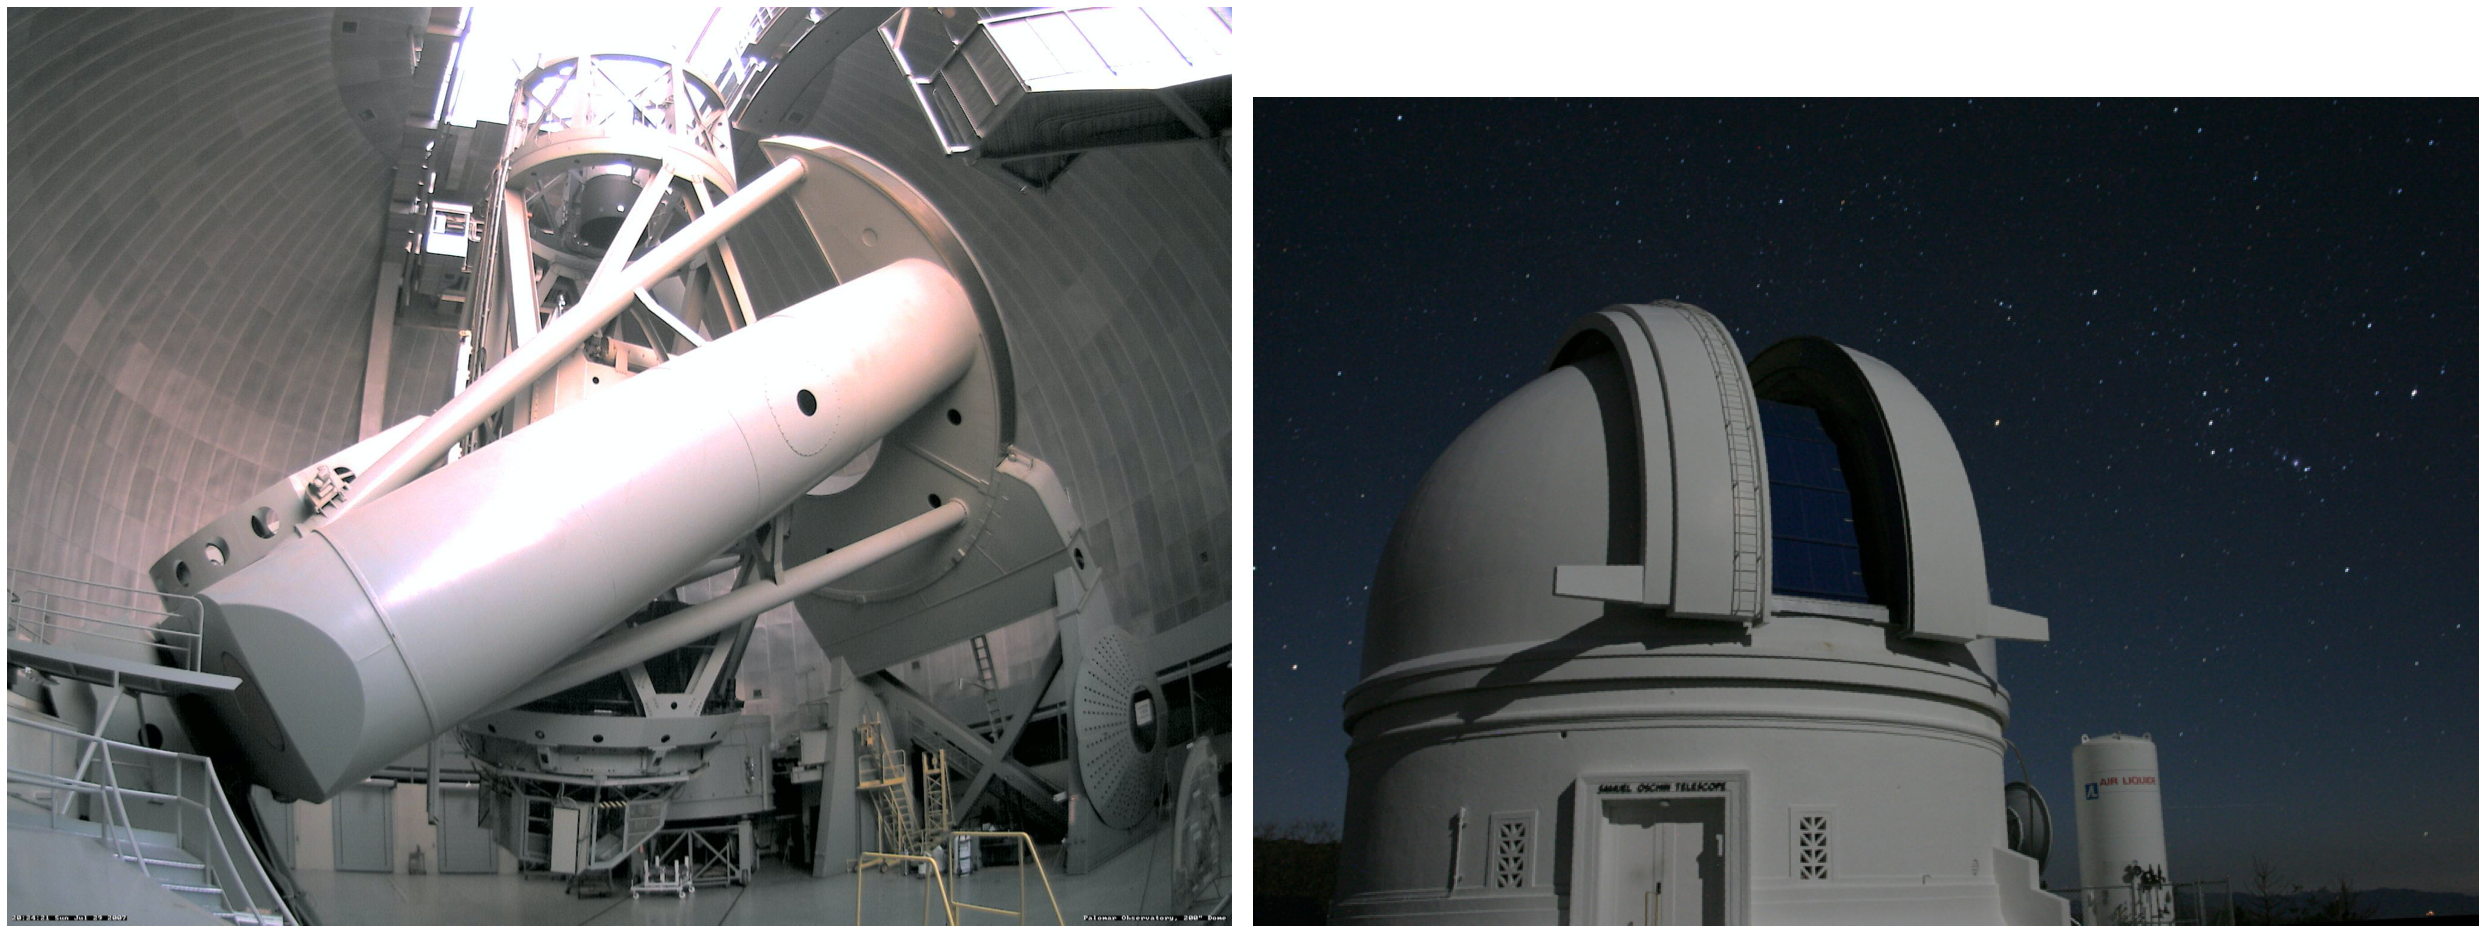
\includegraphics[width=0.75\textwidth]{../figures/02_ztf/p48.png}
  \caption{Télescope Samuel Oshin P48 au Mont Palomar}
  \label{fig:p48}
\end{figure}


\begin{figure}[h]
\centering
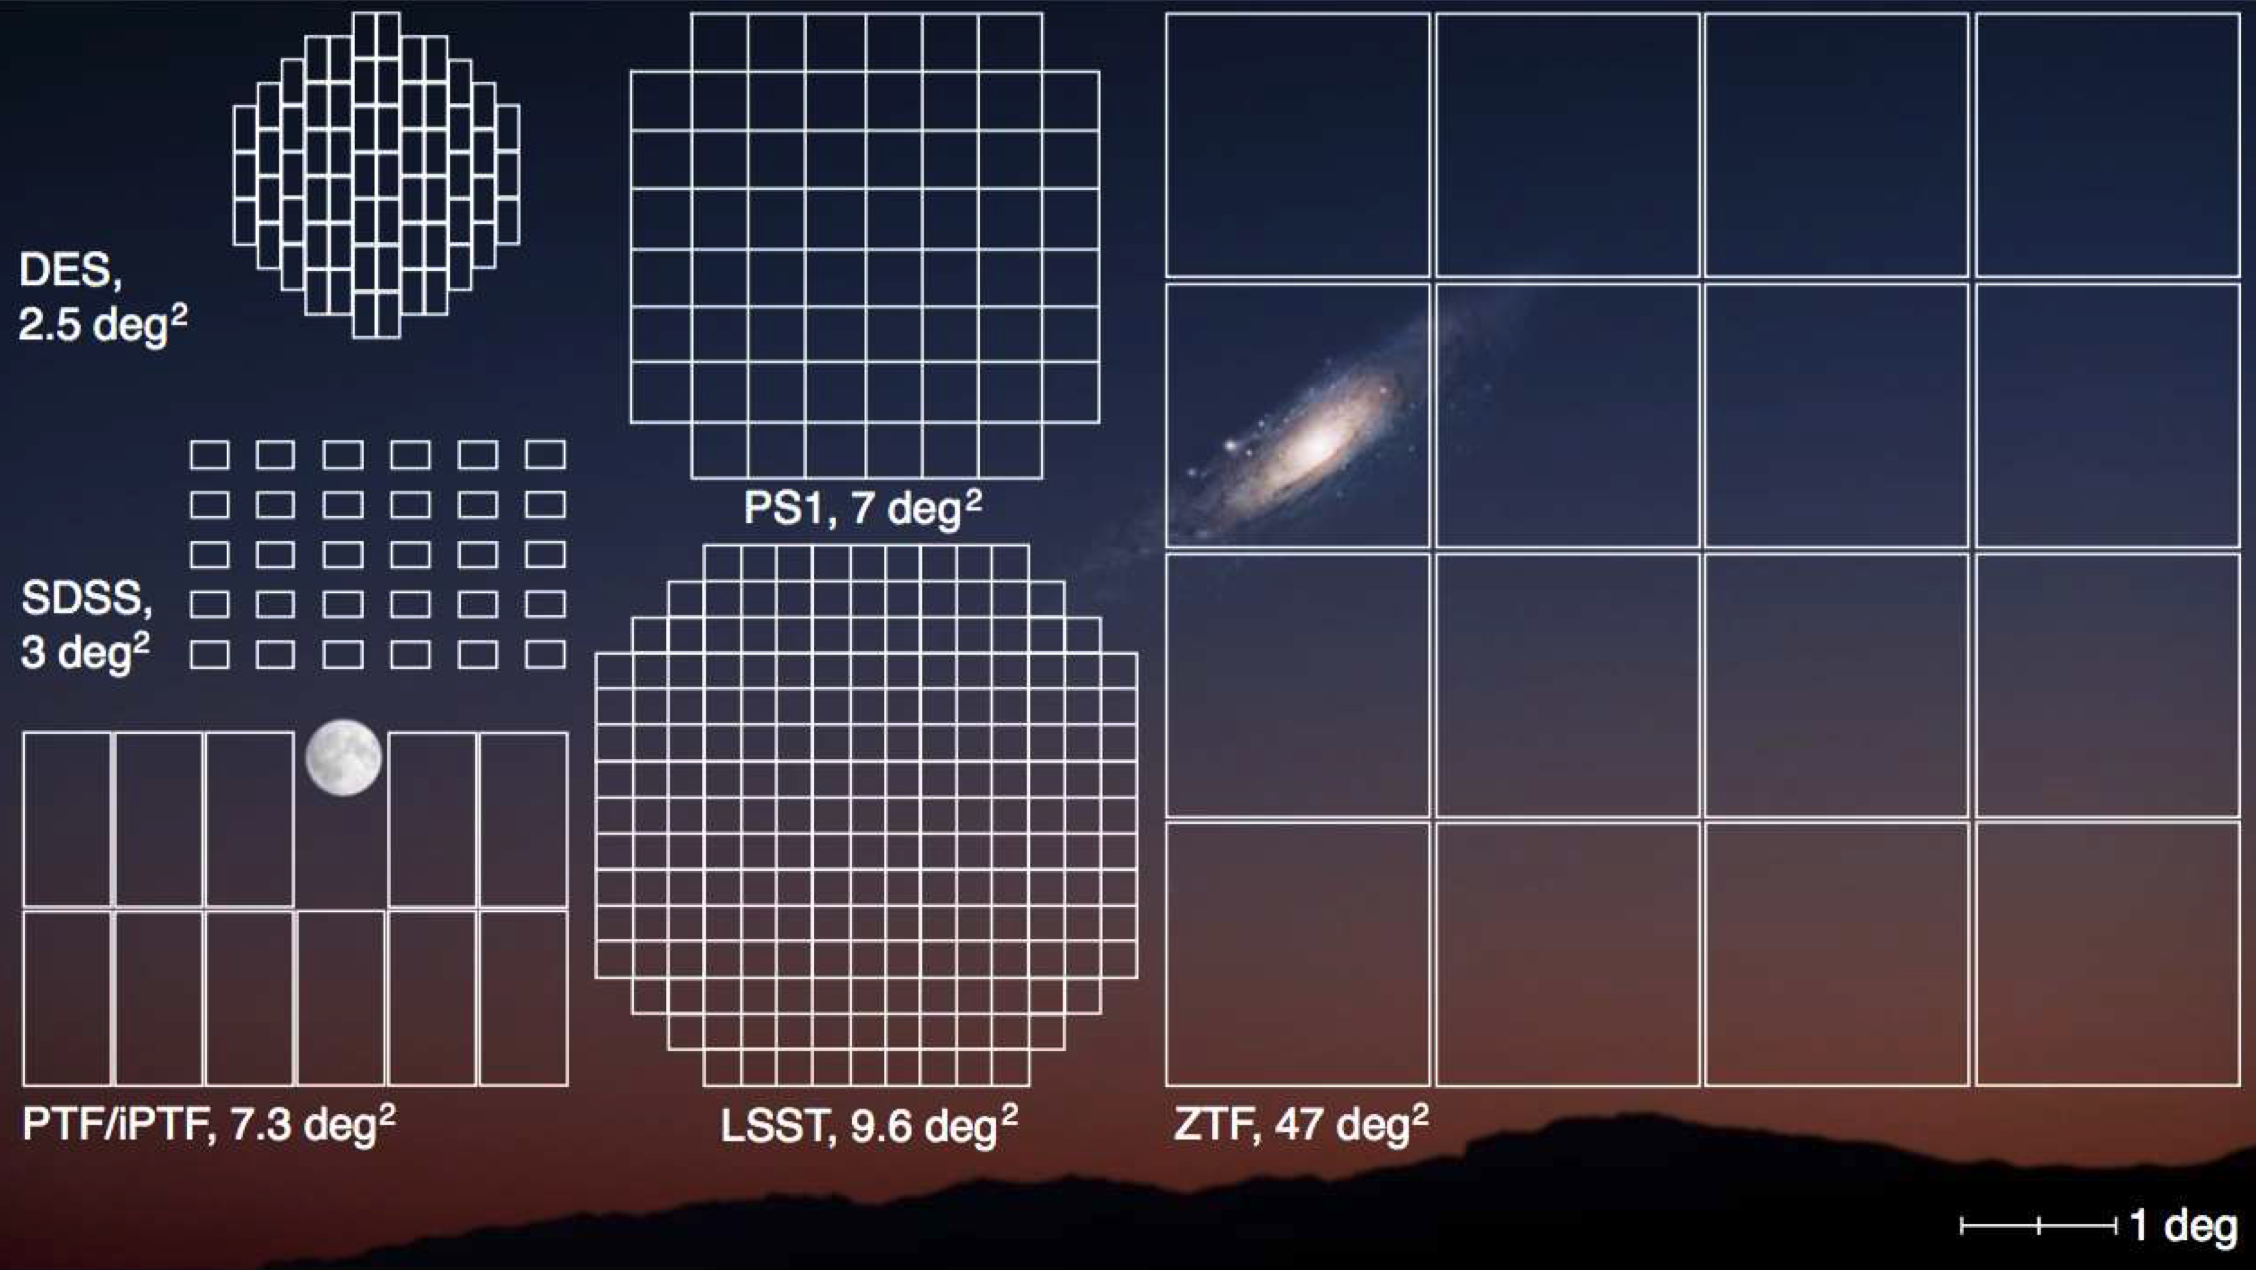
\includegraphics[width=0.9\textwidth]{../figures/02_ztf/ztfcamerafov.png}
\caption{Champ de vue de la caméra ZTF comparé à celui d'autres relevés astronomiques }
\label{fig:ztfcamerafov}
\end{figure}

ZTF est une collaboration internationale financée entre
la US National Science Foundation (NSF) à travers le  programme Mid-scale
Innovations Program (MSIP), et un grand nombre de consortium
internationaux d'Universités et institutions:

\begin{multicols}{2}
\begin{itemize}[noitemsep, label=$\bullet$]
    \item IN2P3\footnote{Institut national de physique nucléaire et de physique
    des particules}.
    \item TANGO University System of Taiwan
    \item Weizmann Institute of Science, Israel
    \item Oskar Klein Center, University of Stockholm, Sweden
    \item DESY/Humboldt University of Berlin, Germany
    \item Ruhr University Bochum, Germany
    \item University of Warwick, UK
    \item Trinity College Dublin, Ireland
    \item University of Maryland, College Park
    \item Northwestern University
    \item University of Wisconsin, Milwaukee
    \item Lawrence Livermore National Laboratory
    \item Caltech/IPAC
\end{itemize}
\end{multicols}

ZTF est ainsi un partenariat privé-public, où son temps d'observation
est divisé pour chaque phase du projet entre trois niveaux:

Lors de la phase 1, le temps d'allocation public (NSF) était de 40\%,
pour les partenariats privés de 40\% également, et les 20 derniers \%
dédiée aux programmes de Caltech qui possèdent l'Observatoire du Mont
Palomar.

L'IN2P3 étant devenu un partenaire majeur de la collaboration, la phase 2
de ZTF a vu un rééquilibrage avec 50\% du temps d'observation attribué
au programme MSIP, et 30\% aux partenaires privés.

Durant le temps d'observation public, ZTF effectue deux sondages distincts: le ciel
Nord d'une part à haute cadence, qui est entièrement scanné tous les trois jours dans les
filtres $g$ et $r$, et le plan
Galactique d'autre part (lattitude $|b|<7\degree$), qui lui est entièrement observé chaque nuit
également dans les filtres $g$ et $r$.

Ces deux sondages combinés mènent à la détection et la génération
d'alertes automatiques de plus d'un million d'évènements par nuit. Ces
évènements sont des phénomènes astrophysiques transitoires ou variables,
dont la magnitude de détection est inférieur à $r\approx 20.5$.

\subsection{Organisation de la recherche scientifique}

Les sections de recherches scientifiques au sein de ZTF sont nombreuses \citep{GrahamZTF2019}:

\begin{itemize}[label=$\bullet$]
\setlength\itemsep{1em}
    \item \underline{L'étude des AGN \& TDEs}:
  
      Les AGN (\textit{Active Galactic Nuclei}), correspondent à une
      région particulièrement lumineuse au coeur des galaxies. Ce sont
      habituellement des trous noirs
      supermassifs et leur disque d'accrétion. Les TDEs, ou \textit{Tidal Disruption Events}, correspondent à des
      phénomènes extrèmement lumineux émanents de cette région.

    \item \underline{L'étude des Supernovae comme sonde cosmologique}
      
      C'est l'utilisation de leur caractéristique de chandelle standardisable pour
      effectuer des mesures précises de distance dans l'Univers
      proche. Avant 2018, seulement $\approx500$ de ces évènements ont
      été observés dans l'Univers proche. En 3 ans ZTF a déterminé près
      de $3000$ distances de ces évènements.

    \item \underline{Physique des Supernovae}

      Indépendamment de leur type, de nombreux mystères demeurent sur la
      physique même de l'explosion des Supernovae. ZTF permet d'obtenir
      un échantillon unique de plusieurs milliers de Supernovae tout
      type confondu qui permet au groupe Bright Transient Survey
      (BTS) d'obtenir des mesures non-biaisées de taux de Supernovae, de fonctions de
      luminosités, de propriétés de galaxies hôte etc.

    \item \underline{Voie Lactée et M31}

      Avec l'observation de plusieurs millions d'étoiles chaque nuit, tout un
      pôle d'étude s'est formé autour des objets internes à notre
      galaxie, mais également dans la galaxie voisine M31, plus connue
      sous le nom d'Andromède. Cet échantillon gigantesque est utilisé pour étudier
      des naines blanches dont la luminosité varie périodiquement,
      d'autres avec des débris transitoires, les systèmes binaires avec
      émission de rayons-X, et de nombreux autres objets stellaires.


    \item \underline{L'Astrophysique Multimessager}

      Cette toute nouvelle branche de la physique a vue le jour notamment grâce aux
      premières détections d'ondes gravitationnelles ou de neutrinos. De
      tels phénomènes sont habituellement grossièrement localisés avec
      la détection de ce type de signal, ce qui rend difficile
      l'identification de la source. Dans le cas où une contrepartie
      électromagnétique existe, ZTF est alors capable de compléter la
      détection primaire avec une observation photométrique aux prémices de
      l'évènement, notamment grâce à son champ de vue extrêmement
      large et sa haute cadence.

    \item \underline{Corps au sein du système Solaire}

      Ce groupe se concentre sur la découverte et la caractérisation des
      petits corps au sein de notre système solaire, à savoir des
      astéroïdes, des comètes etc.
\end{itemize}

La répartition du temps d'observation pour ces différents champs de
recherches est adaptée de la façon suivante \citep{Bellm19b}:

\begin{itemize}[label=$\diamondsuit$]
  \itemsep0em 
\item L'étude des corps au sein
  du système solaire se fait principalement durant l'aube et l'aurore
  ($\sim3.5\%$ du ciel pour chaque et principalement en bande $r$).
\item L'étude de la physique des Supernovae bénéficie d'une observation
  haute cadence (3 jours dans $g$ et $r$) de $\approx1800\text{deg}^{2}$, et qui correpond à une
  allocation de $15\%$ du temps d'observation. 
\item  $\approx8\%$ du temps pour la Cosmologie dans le ciel extra-galactique.
\item Le groupe Galaxy Science observe la Voie Lactée principalement en
  été ($\approx5\%$, toutes bandes confondus).
\item Le groupe Astrophysique multi-messager peut observer et étudier de
  potentiels sources pour $\approx5\%$ du temps (toutes bandes confondus)
\end{itemize}

\begin{figure}[h]
  \centering
  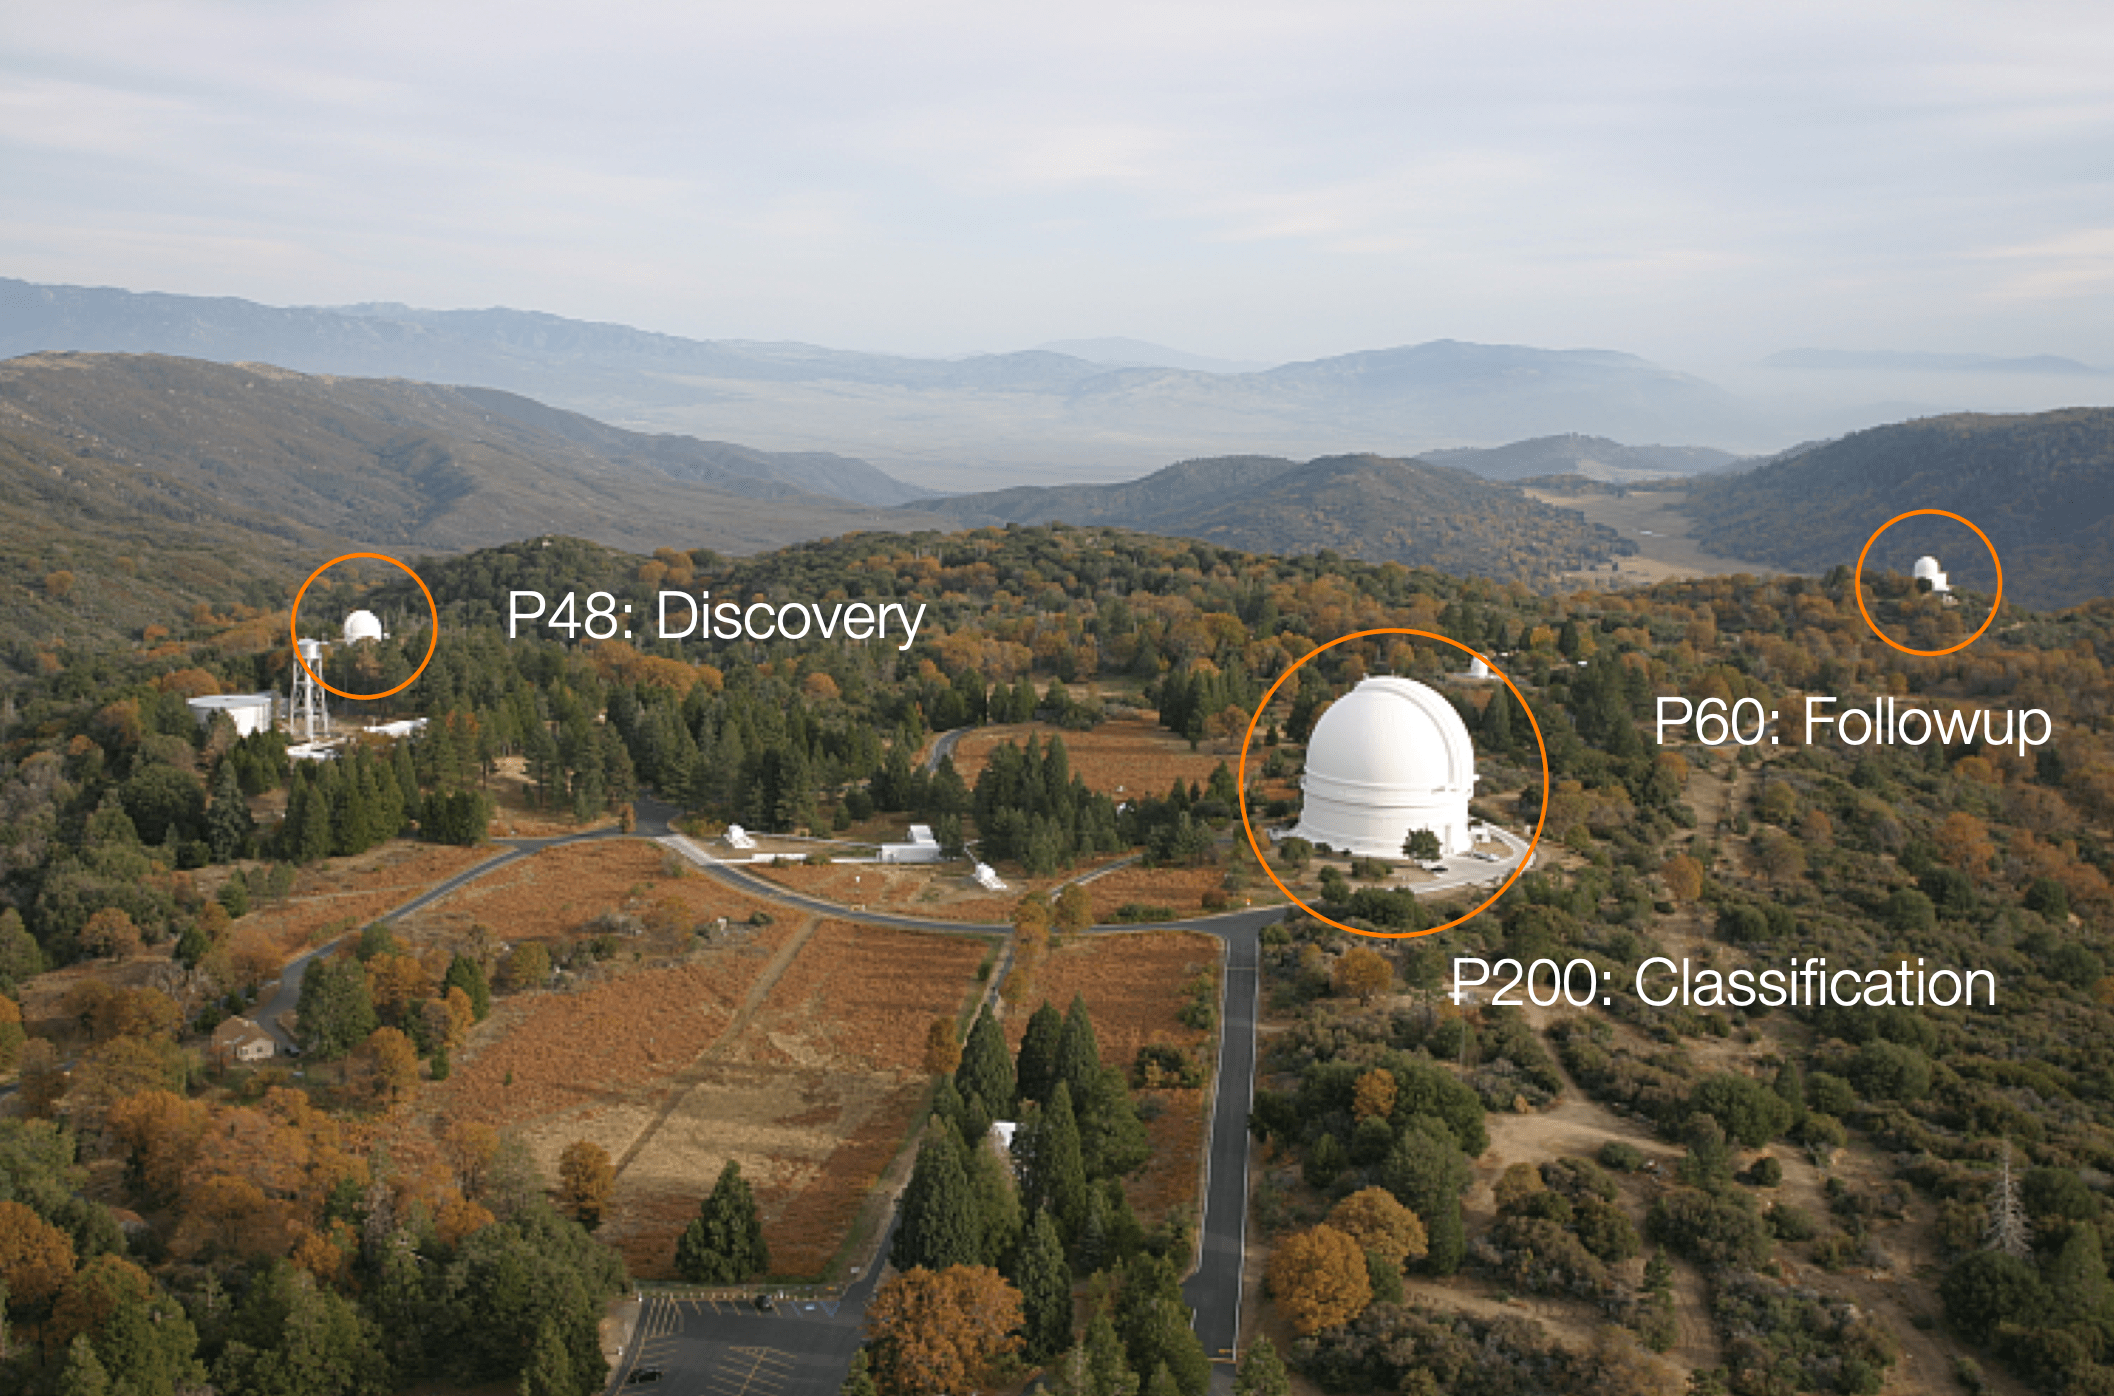
\includegraphics[width=0.75\textwidth]{../figures/02_ztf/palomar_obs-min.png}
  \caption[Observatoire de Palomar]{Observatoire de Palomar, en Californie. Sur la gauche est
    située la caméra principale de ZTF, attachée au télescope P48 Samuel
    Oschi. En haut à droite nous avons le P60, sur lequel est monté le
    spectrographe 3D SEDm appartenant également à la collaboration
    ZTF. Le P200 est quant à lui utiliser par de nombreuses
    collaborations, et est utilisé occasionnellement par ZTF.}
\label{fig:palomar_obs}
\end{figure}

\section{La caméra ZTF}
\label{sec:ztfcamera}

\subsection{Caractéristiques}

La nouvelle configuration de ZTF vis à vis de ses prédecesseurs PTF/iPTF
est principalement due à sa nouvelle caméra de $47\text{deg}^{2}$, profitant de
l'intégralité du plan focal du télescope Schmidt P48.

Comme illustré dans la Fig.~\ref{fig:ztfcamera} de \citet{BellmZTF2019}, la caméra est
constituée d'une mosaïque de 16 CCD (Charge Coupled Device) composés de
pixels carrés de \SI{15}{\micro\metre} de côté, à une échelle de $1\farcs01$
$\text{pixel}^{-1}$. Chaque CCD est composé de 6144$\times$6160 pixels,
et la caméra dans son ensemble a donc 573 Mpx. 


\begin{figure}[ht]
\centering
\subfloat[Plan focal de la caméra ZTF \citep{BellmZTF2019}.]{\label{fig:ztfcamera}{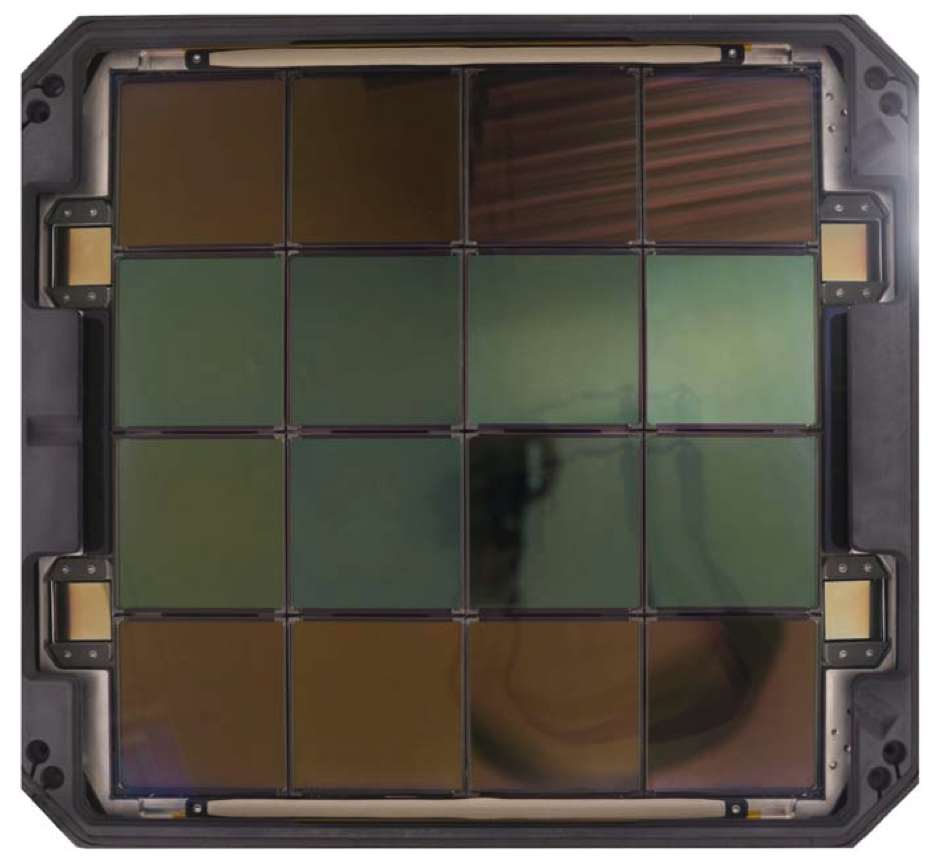
\includegraphics[width=0.4\textwidth]{../figures/02_ztf/ztfcamera.png}}}\hfill
\subfloat[Vue en coupe du télescope Samuel Oschin avec le nouveau
système ZTF \citep{DekanyZTF2020}.]{\label{fig:p48details}{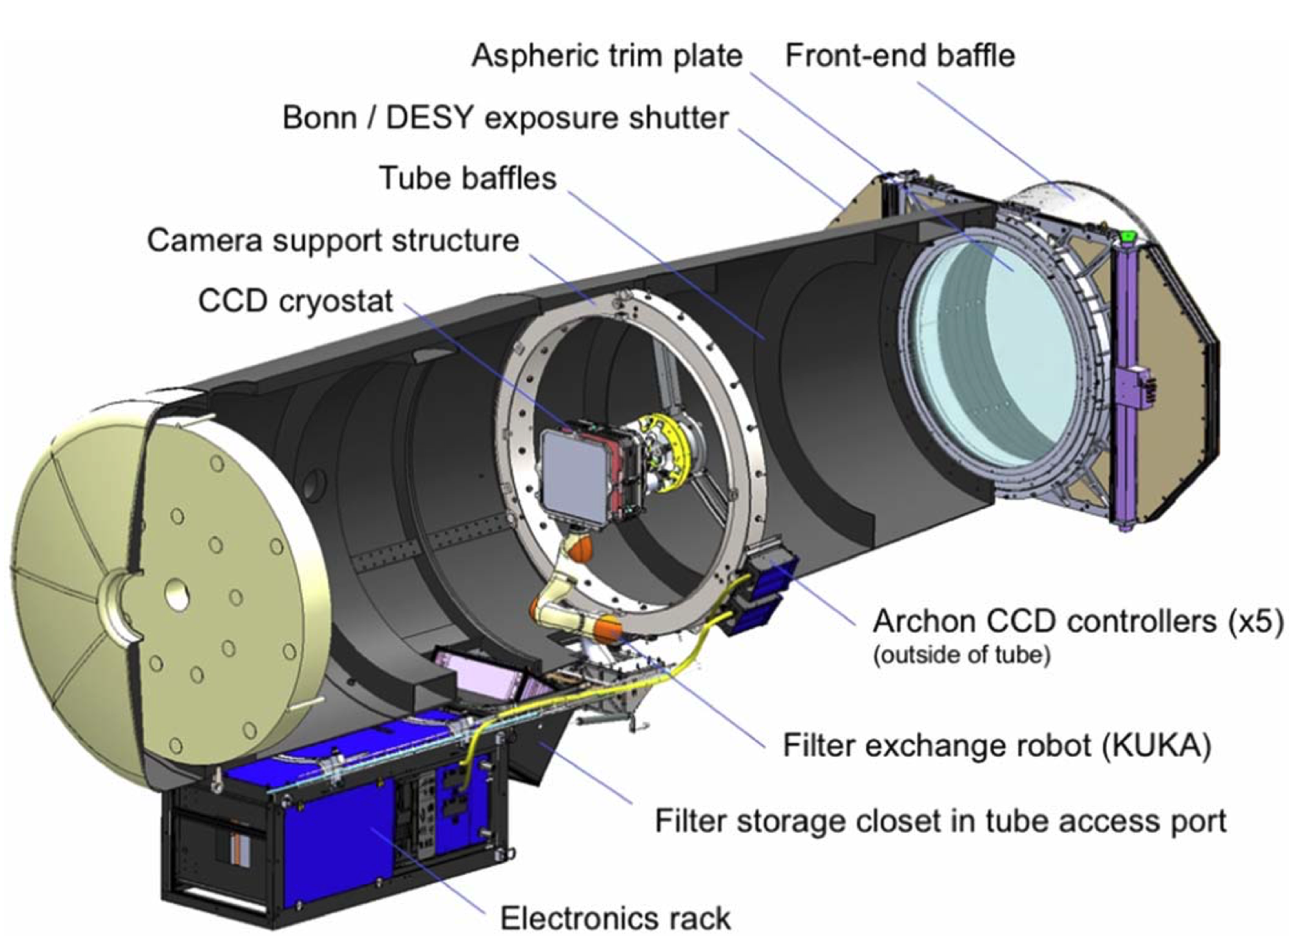
\includegraphics[width=0.5\textwidth]{../figures/02_ztf/p48details.png}}}
\caption[Système d'imagerie ZTF et caméra]{Description du système d'imagerie de ZTF (\textit{à droite}) et présentation du
  plan focal de la caméra et ses 16 CCD (\textit{à gauche}). }
\label{fig:imageriecamztf}
\end{figure}


La FWHM mediane de la fonction d'étallement du point
(PSF) résultant de cette configuration est de $2\farcs1$ dans les bandes
$g$ et $i$, et de $2\farcs0$ dans la bande $r$. Leur transmission
respectives est présentée dans la Figure~\ref{fig:ztffilters}. En ce qui concerne la limite en magnitude, la bande $g$ montre un seuil median à
$5\sigma$ de $20.8$mag, la bande $r$ de $20.6$mag et la bande $i$
$19.9$mag. Nous illustrons les distributions de la FWHM et du seuil en
magnitude pour chaque filtre dans la Figure~\ref{fig:ztfperffilts}. 


\begin{figure}[ht]
  \begin{minipage}[c]{0.55\textwidth}
    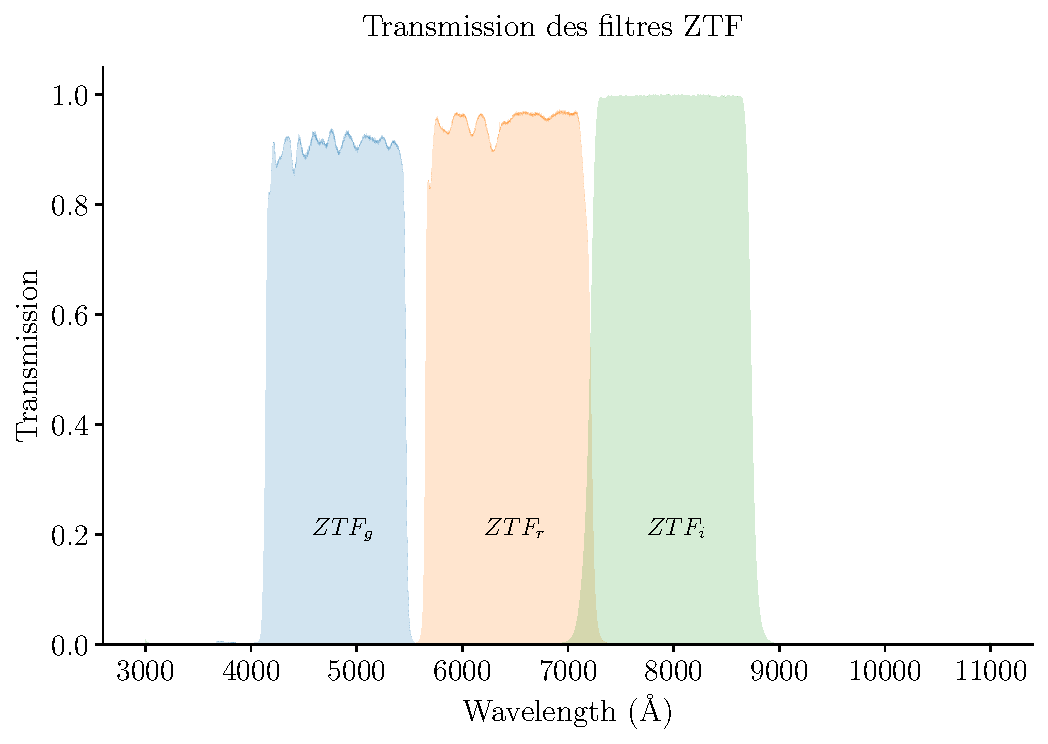
\includegraphics[width=\textwidth]{../figures/02_ztf/ZTFfilters.pdf}
  \end{minipage}\hfill
  \begin{minipage}[c]{0.45\textwidth}
    \caption[Transmission des filtres $g$, $r$ et $i$ de
    ZTF]{Transmission des filtres $g$, $r$ et $i$ de ZTF \citep{DekanyZTF2020}}\label{fig:ztffilters}
  \end{minipage}
\end{figure}



\begin{figure}[h]
  \centering
  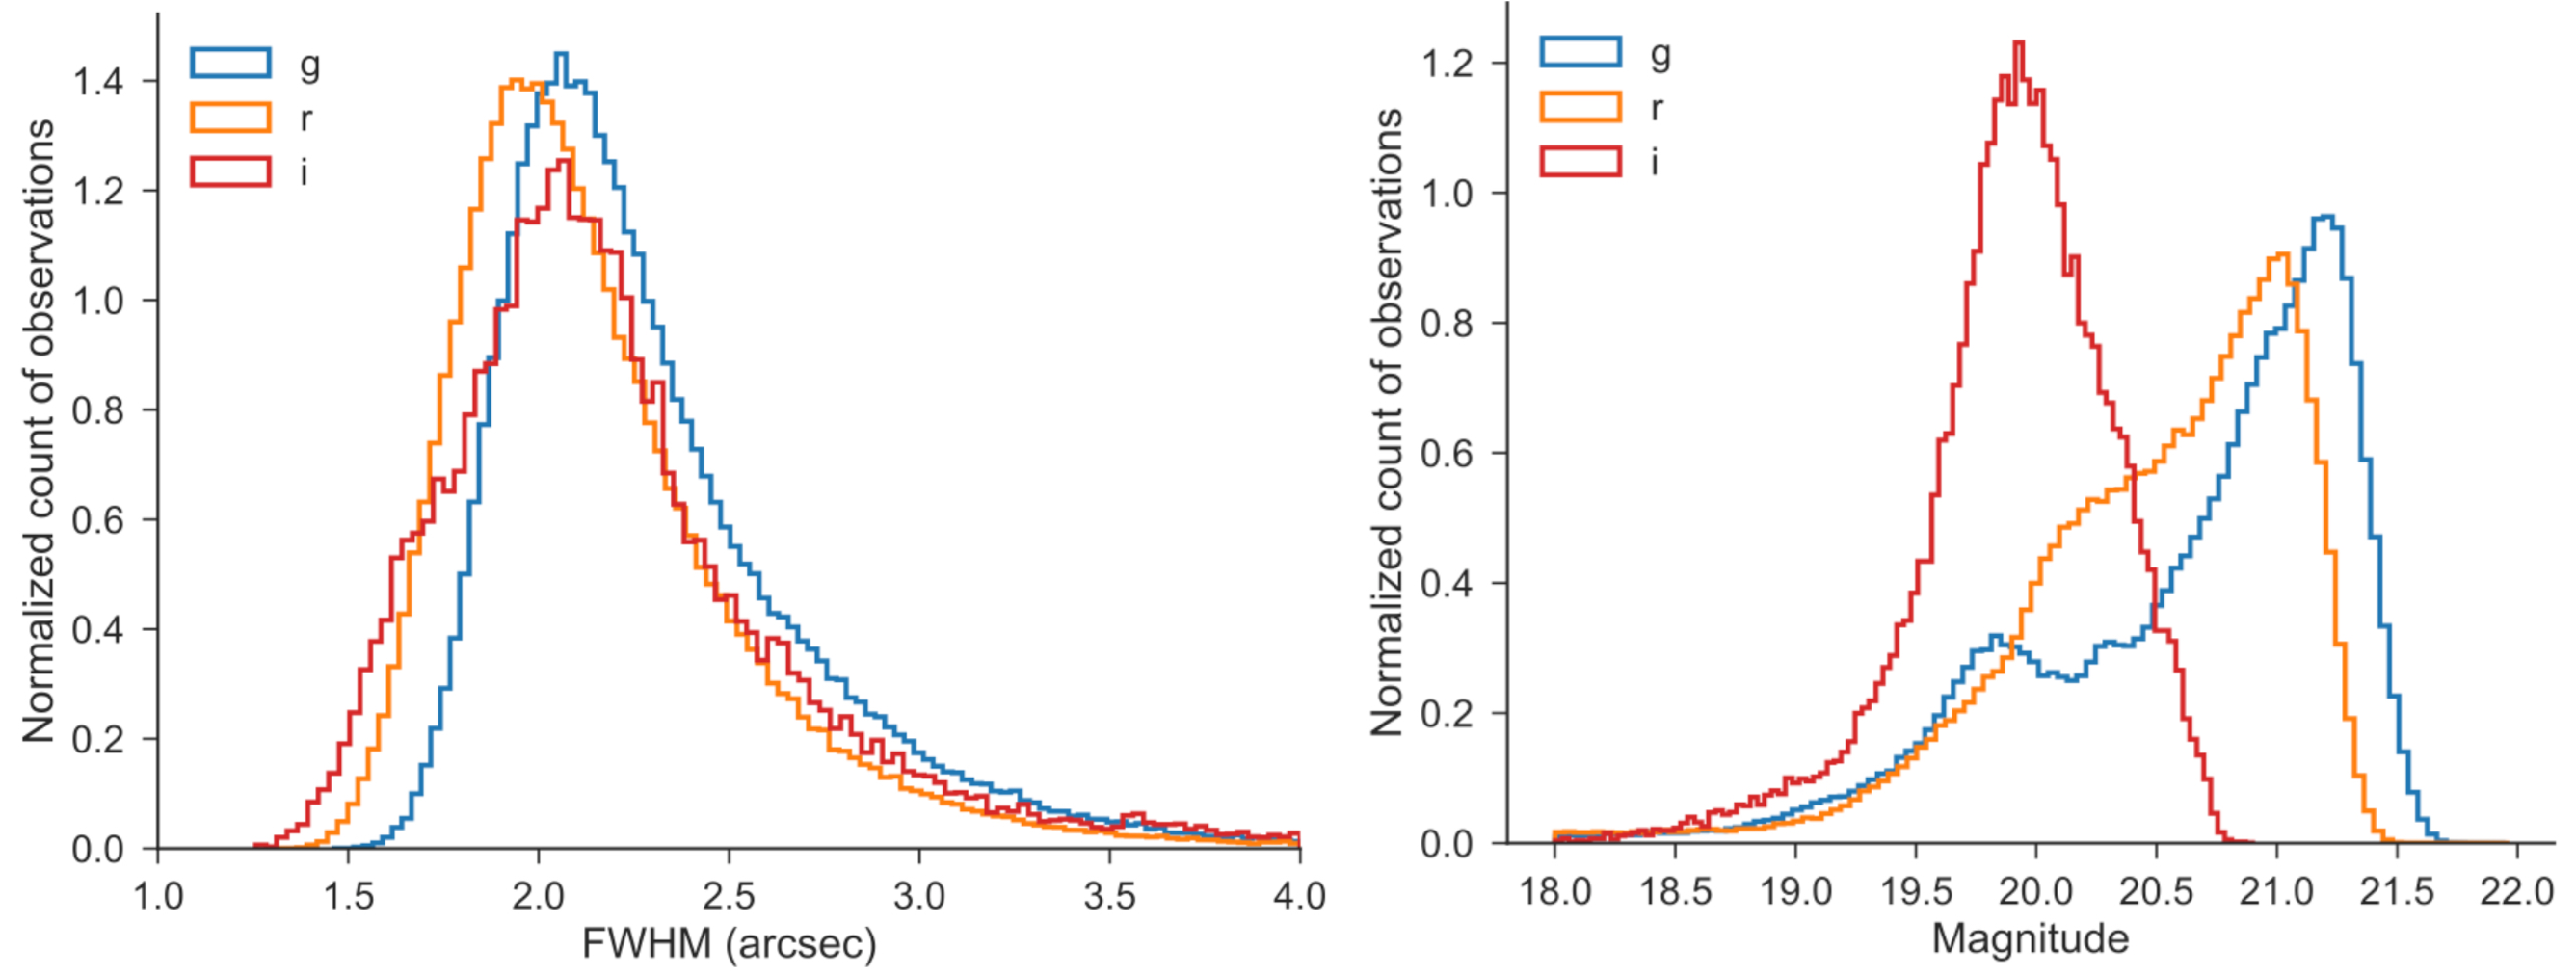
\includegraphics[width=0.99\textwidth]{../figures/02_ztf/ztfperformances.pdf}
  \caption[Profondeurs et FWHM associées aux filtres de la caméra
  ZTF]{\textit{À gauche} l'histogramme
    normalisé de la largeur à mi-hauteur (FWHM) de la fonction
    d'étalement de point (PSF) pour chaque filtre durant le mois de Juin
    2018 \citep{BellmZTF2019}. \textit{À droite} est représenté
    l'histogramme à $5\sigma$ des magnitudes limites avec un temps de
    pose de $30s$ pour chaque filtre sur une période d'une lunaison.}
  \label{fig:ztfperffilts}
\end{figure}


Le temps de pose utilisé avec cette caméra est de $30s$, et la vitesse
de lecture de seulement $8s$. Entre le champ de vue de
$47\text{deg}^{2}$ et cette haute cadence d'acquisition, ZTF est capable
de scanner près de $3750\text{deg}^{2}$ par heure. Sachant que tout au long
de l'année il y a en moyenne 6h de ciel noir par nuit au Mont Palomar, ZTF est ainsi
capable d'observer l'entièreté du ciel visible plus d'une fois par
nuit. Pour donner un autre
ordre d'idée, ZTF serait ainsi capable de reproduire le relevé POSS
\citep{MinkowskiPOSS} en 2 nuits.


\subsection{Gestion des données}

Bien évidemment, un tel flux de données nécessite une infrastructure de
traitement adéquate. Celle ci, appelée ZTF Science Data System (ZSDS)
est hébergée à l'IPAC\footnote{Infrared Processing \& Analysis Center: \href{https://
www.ipac.caltech.edu}{https://www.ipac.caltech.edu}} \citep{MasciZTF2019}. Ce système
comprend le traitement des données, l'infrastructure
d'émission d'alertes, le système d'interface utilisateur pour l'accès
et l'analyse des résultats. Ce pipeline (exécuté en temps réel) utilise
un algorithme de différentiation d'image, optimisé pour la détection de
point source variable ou transitoire. Une fois l'évènement confirmé, une alerte est générée et
en générale déployée dans le quart d'heure qui suit. La distribution de
ce flux d'alertes utilise des technologies dont le code source est
public et qui sont développées
en industries: Apache Kafka\footnote{\url{https://kafka.apache.org}} qui
fourni un système unifié en temps réel à latence faible pour la
manipulation de flux de données, et
Avro\footnote{\url{https://avro.apache.org}} qui est un framework de
sérialisation de données. Les ordres de grandeurs de la quantité de
données à manipuler sont impressionnants: Ce système gère avec succès un
flux d'environ $1,2$ millions d'alertes ($\sim$ $70$ GB de données) par
nuit. La vitesse de transfert est d'environ $80,000$ alertes/minute. Plus
de détails sur le système de distribution d'alertes sont apportés dans
\citet{PattersonZTF2019}. On notera que le framework Avro sera celui utilisé
pour LSST.

Seules les alertes provenant des observations liées au programme MSIP
sont rendues public immédiatement. Les images en revanches (brut,
calibrées et produits de données associés) deviennent disponibles 6 à 12 mois 
après l'observation pour la Phase 1 de ZTF, et entre 3 et 6 mois pour la
Phase 2. Les données d'observation ayant pour origine les programmes
privés et de Caltech sont disponibles après environ 12 à 18 mois. Lors
de l'écriture de ces lignes en Avril 2022, la
DataRelease\footnote{\url{https://www.ztf.caltech.edu/ztf-public-releases.html}}
10 est public, ce qui correspond à toutes les observations MSIP de Mars 2018 au 5 Novembre
2021, et celles privées et de Caltech jusqu'au 5 Juillet 2020.

\section{Observation des Supernovae Ia avec ZTF}\label{sec:sniaztf}

Nous allons à présent nous focaliser sur l'observation des Supernovae de
type Ia avec ZTF.

Les évènements transitoires nécessitant d'être filtrés parmis toutes les
alertes reportées par ZTF, \citet{NordinAMPEL2019} a élaboré le système
\pkg{AMPEL}\footnote{\url{https://github.com/AmpelProject/Ampel-contrib-sample}} afin d'automatiquement filtrer
les détections de ZTF et établir les courbes de luminosité associés aux
évènements retenus.

Sur les $\sim 10^{5}$ alertes par nuit (ce qui correspond environ à
$10\%$ de ce qui est attendu pour LSST), la majorité ($\sim 90\%$)
d'entre elles sont filtrés comme étant des artefacts, des étoiles
variables, des satellites ou encore des objets du système solaire. In
fine, ''seulement'' $\mathcal{O}(10)$ sont de nouvelles Supernovae qui
doivent être identifées et classifiées. Entre $70$ et $80\%$ d'entres
elles s'avèrent être de type Ia, dont la moitié atteignent le seuil de
magnitude de ZTF permettant d'établir une courbe de lumière
exploitable.

La $1\iere{}$ data release dédiée au sondage des Supernovae de type Ia
avec ZTF a été publiée et décrite par \citet{DhawanZTFDR1} très
récemment. Au stade de cette DR1, ce qui correspond à un peu plus de 2
ans et demi d'observations (Mars 2018-Novembre 2020), ZTF a déjà
répertorié plus de $3000$ SNIa.

La profondeur en magnitude atteint
$20.8$, $20.6$, $20.3$ mag dans les bandes $g$ $r$, et $i$ respectivement, ce qui
correspond à un redshift $z\lesssim0.1$. L'échantillon est complet à
$100\%$ en terme de classifcation en deça de $m_{peak}=16.5$ mag, à
$93.6\%$ en deça de $m_{peak}=18.5$ mag et $88.8\%$ à $m_{peak}=19.0$
mag \citep{FremlingZTFspec2020}.

Cette classification est rendue possible grâce à la combinaison de la
caméra de ZTF et du spectrographe 3D monté sur le P60, la Spectral
Energy Distribution machine (SEDm), qui est optimisé pour la
classification des SNe jusqu'à $m\approx19$ mag. Nous détaillerons cet instrument
dans le chapitre suivant. La DR1
présente ainsi un échantillon de $761$ Supernovae classifiées
spectralement avec un redshift median de $\overbar{z}=0.057$, incluant $547$ SNeIa, $155$ SNeII, $40$ SNeIb/c et $19$ SLSNe.
La Figure~\ref{fig:cumulsniaztf} (\textbf{Rigault et al DR2}) met en évidence la croissance de
l'échantillon de SNeIa observées durant la phase 1 de ZTF, qui
constituera la $2\ieme$ Data Release de ZTF-Cosmo consacrée aux Supernovae de
type Ia.

Sur les $\approx3700$ SNeIa classifiées spectralement, près de
$3000$ entrent dans la catégorie \textit{échantillon dorée}, ce qui
signifie qu'elles remplissent les critères dit de qualité cosmologiques
pour leur courbe de luminosité vis à vis de l'algorithme SALT2 qui en
dérive les paramètres de couleur et de stretch. Ces
critères, basés sur l'intervalle de phase $[-15,30]$ jours où SALT2 est
le mieux définie, sont les suivants:

\begin{itemize}[label=$\diamondsuit$]
  \itemsep0em 
   \item Seulement les détections photométriques à $5\sigma$ sont
     considérées
   \item Au moins $7$ points avec le maximum dans au moins $2$ bandes
   \item Au moins $7$ points après le maximum dans au moins $2$ bandes
\end{itemize}

Environ $40\%$ de ces Supernovae possèdent un redshift spectral de leur
galaxie hôte (majoritairement des relevés SDSS). $50\%$ proviennent des
caractéristiques des spectres des supernovae elles mêmes, et $10\%$ de
raies d'émissions de la galaxie hôte ayant contaminées le spectre de la
SNIa. Il est à noté que pour les 2 derniers points, la précision n'est
que de l'ordre de $5$\textperthousand, insuffisant pour la cosmologie.
Cependant, plus de $95\%$ des galaxies hôtes ont une magnitude supérieur
à $20$ mag, ce qui signifie que d'autres relevés (comme par exemple
DESI) pourraient à posteriori mesurer et fournir les redshift manquant.

\begin{figure}[h]
  \centering
  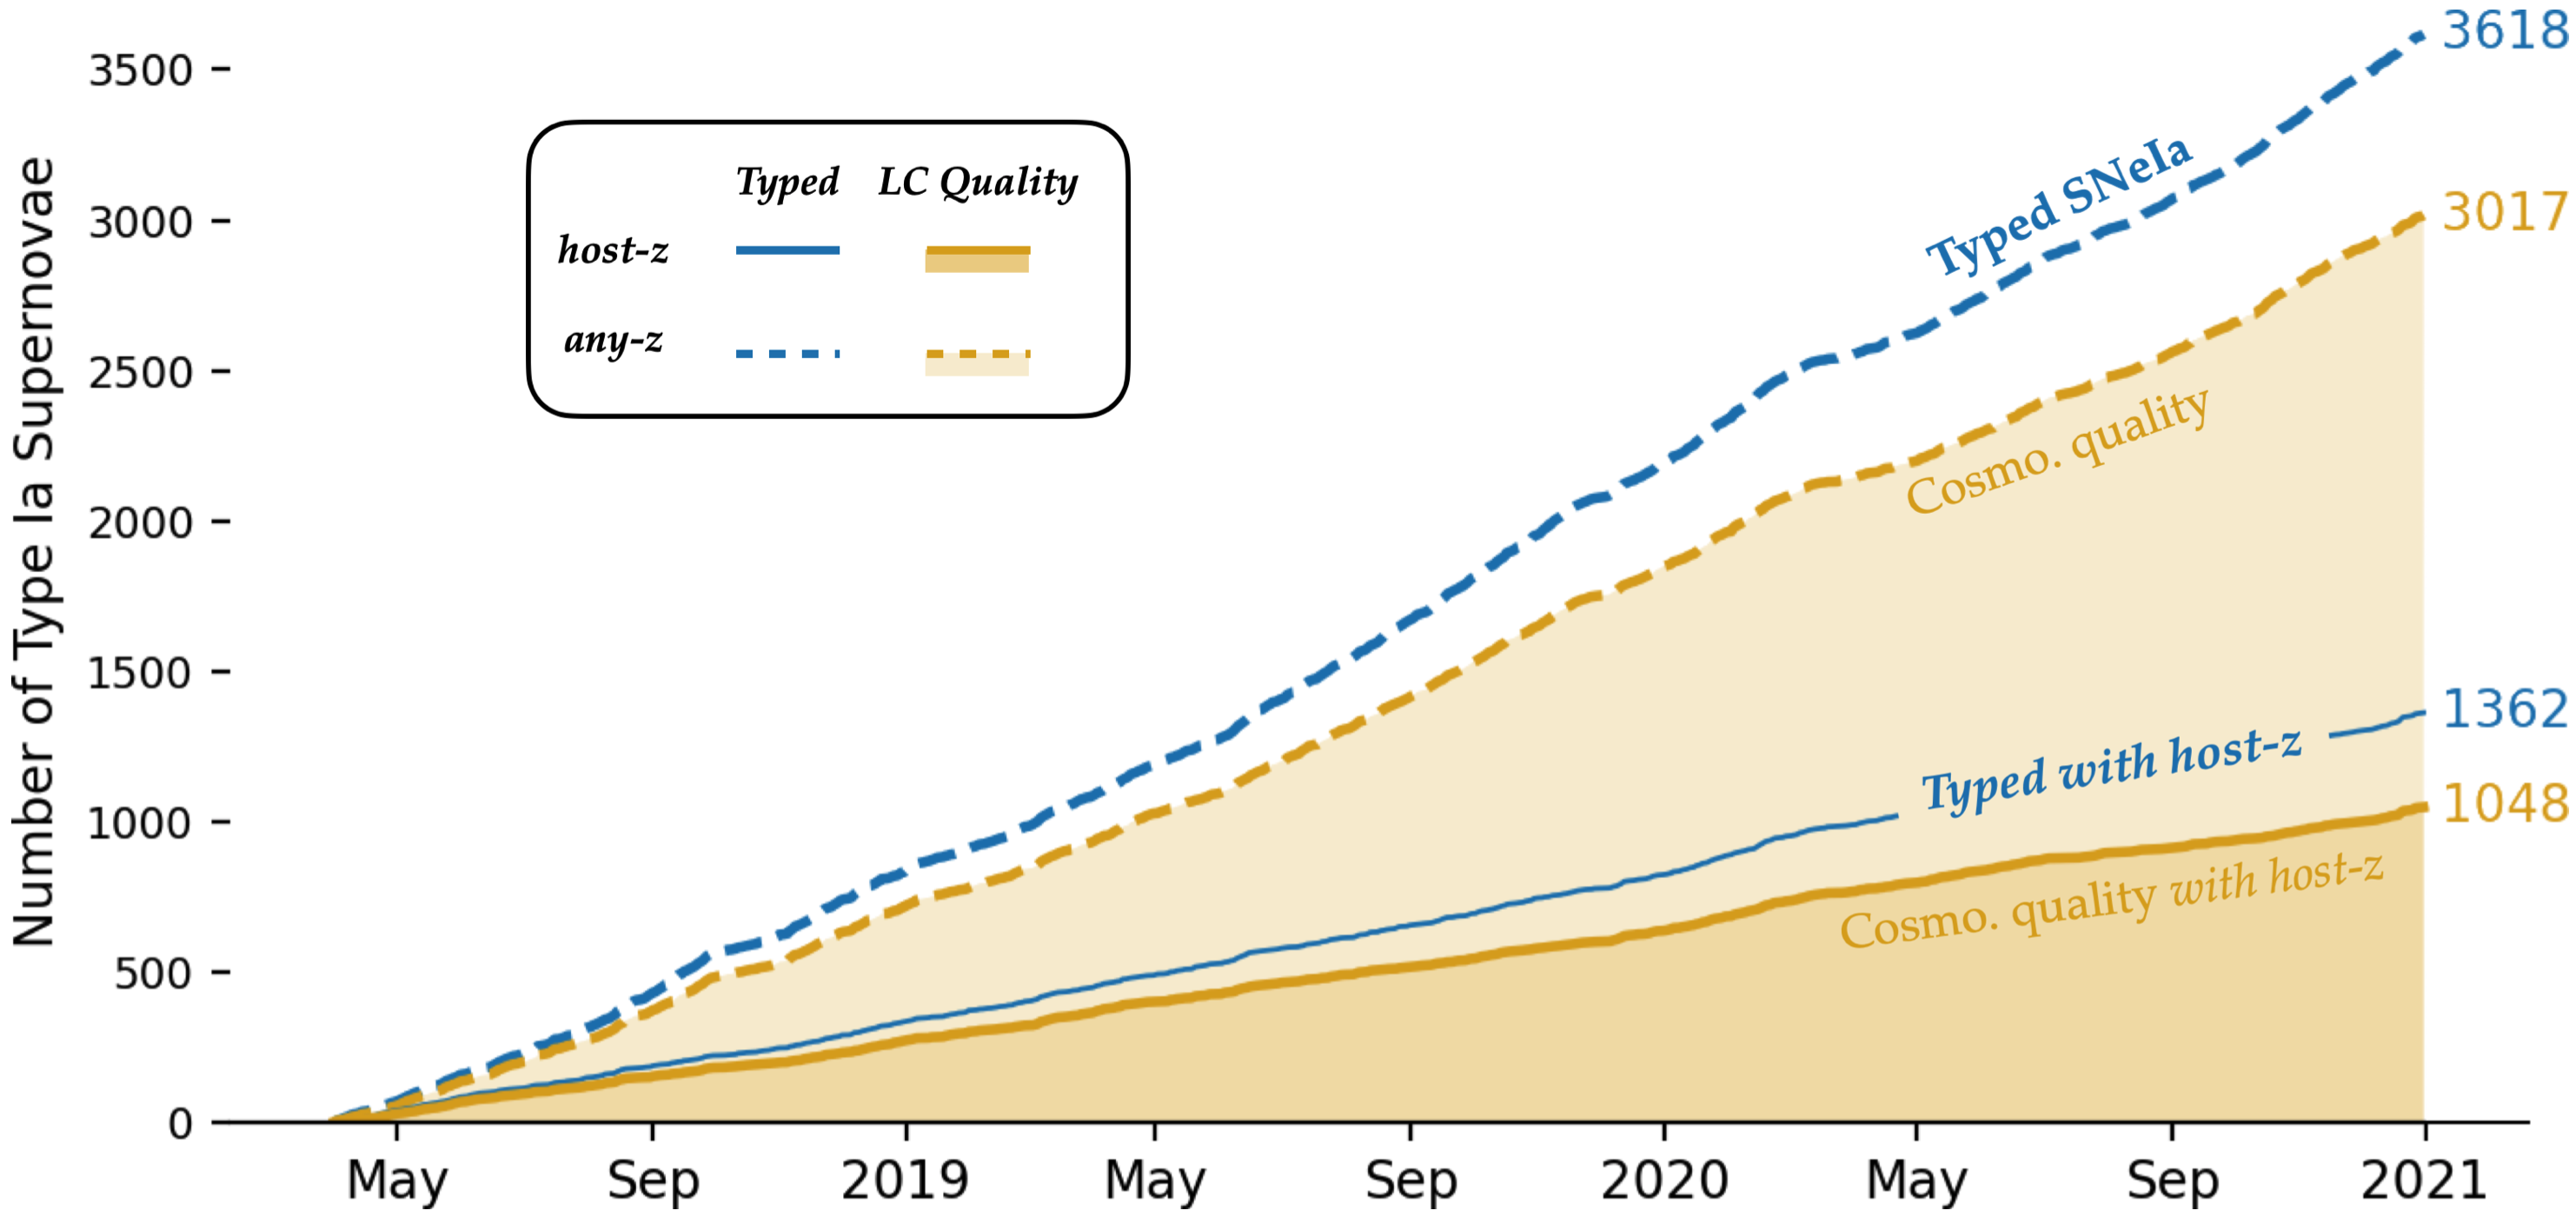
\includegraphics[width=0.99\textwidth]{../figures/02_ztf/cumulsniaztf.png}
  \caption[Nombre cumulé de SNIa observés par ZTF (phase 1)]{Nombre
    cumulé de SNIa observés par ZTF (phase 1). Les contours dorés
    correspondent à l'échantillon passant les critères de coupure pour
    une qualité cosmologique. Le trait plein montre les SN avec un
    redshift spectroscopique de leur galaxie hôte. À titre de
    comparaison, le set de données le plus récent dans la littérature
    cosmologique comptabilise moins de $500$ SNIa à un redshift de $z<0.1$}
  \label{fig:cumulsniaztf}
\end{figure}

ZTF a donc montré sa capacité à débusquer et classifier pas moins de
$1000$ Supernovae de type Ia par an, très loin devant l'actuel (ancien)
leader à bas redshift Pantheon \citep{Scolnicpantheon18} avec 1048 SNeIa
sur les 20 dernières années, dont seulement 210 à un redshift
$z<0.1$. Leur plus récente publication
\citep[Pantheon+,][]{Scolnicpantheon21} fait état de 1550 SNeIa, dont 389 à $z<0.1$.

Nous parlerons dans le dernier chapitre de ce manuscrit de la nouvelle
Data Release 2 actuellement en cours d'étude, des premiers résultats obtenus sur les courbes de
lumières ainsi que des ouvertures sur la dérivation de paramètres
cosmologiques.

Rappelons que la cosmologie avec les SNeIa se base sur la capacité, certes, à
détecter les supernovae grâce à la caméra ZTF, mais également à leur
classification. Cette étape a été peu détaillée dans ce chapitre, mais
est cruciale pour éviter toute contamination des échantillons de SNeIa,
induisant des biais dans la dérivation des paramètres cosmologiques
\citep{JonesScolnic17SNcontam}.

Comme nous l'avons mentionné au tout
début de la Section~\ref{sec:ztfcollab}, cette classification se fait
grâce à un spectrographe 3D monté sur le télescope P60. Le chapitre
suivant est tout naturellement dédiée à la présentation de cet
instrument, l'extraction de spectre et sa classifcation.


%\bibliographystyle{../main/aa_url}
%\bibliography{99_references}
\end{document}

%%% Local Variables:
%%% mode: latex
%%% TeX-master: t
%%% TeX-master: t
%%% TeX-master: t
%%% TeX-master: "../main/main"
%%% TeX-master: t
%%% TeX-master: t
%%% TeX-master: t
%%% TeX-master: t
%%% TeX-master: t
%%% TeX-master: t
%%% End:
